\documentclass[12pt,a4]{article} %[font size, tamano de hoja]{Tipo de documento}

\usepackage[left=1.8cm,right=1.8cm,top=32mm,columnsep=20pt]{geometry}

\usepackage[utf8]{inputenc} %Formato de codificación
\usepackage[spanish, es-tabla, es-nodecimaldot]{babel}
\usepackage{amsmath} %paquete para escribir ecuaciones matemáticas
\usepackage{amssymb} %paquete para símbolos adicionales
\usepackage{float} %Para posicionar figuras
\usepackage{graphicx} %Para poder poner figuras
\usepackage{hyperref} %Permite usar hipervínculos 
\usepackage{multicol} %Para hacer doble columna
\usepackage{subcaption}
\usepackage{float}
\usepackage[sorting=none]{biblatex} %Imports biblatex package. To cite use \cite{reference_label}
\addbibresource{tp4.bib} %Import the bibliography file



\title{Aplicación de Métodos Numéricos en la Optimización de Sistemas Lineales"\\


\vspace{20mm}

 Métodos Numéricos y Optimización\\
 Trabajo práctico N$^{\circ}$4\\
}

\author{Timoteo Menceyra y Alejo Zimmermann\\ [2mm] %\\ para nueva línea
\small Universidad de San Andrés, Buenos Aires, Argentina}
\date{1er Semestre 2024}
% Tamanos de letra: 
% \tiny	
% \scriptsize
% \footnotesize
% \small	
% \normalsize	
% \large	
% \Large	
% \LARGE	
% \huge	
% \Huge


%Todo lo que está antes de begin{document} es el preámbulo
\begin{document}
\vspace{1cm} % Ajusta la distancia vertical entre la fecha y la imagen



\maketitle
% \begin{center}
% \includegraphics[width=5cm]{logoUdesa.png} % Ajusta la ruta y el tamaño de la imagen
% \end{center}


\begin{abstract}

Este informe presenta los resultados de experimentos numéricos centrados en la optimización de sistemas lineales utilizando el método de descenso por gradiente. Específicamente, abordamos el problema de encontrar la solución del sistema \(Ax = b\) minimizando la función de costo \(F(x) = (Ax - b)^T (Ax - b)\). El algoritmo de descenso por gradiente busca iterativamente la solución óptima \(x^*\), y exploramos su desempeño en términos de convergencia y precisión. Además, introducimos la regularización L2 para manejar casos donde el problema tiene más incógnitas que ecuaciones, modificando la función de costo a \(F_2(x) = F(x) + \delta_2 \|x\|_2^2\).

Los experimentos se realizaron utilizando matrices \(A\) y vectores \(b\) generados aleatoriamente con dimensiones \(n = 5\) y \(d = 100\), y el parámetro de regularización \(\delta_2 = 10^{-2} \sigma_{max}\). Realizamos 1000 iteraciones del algoritmo de descenso por gradiente con un tamaño de paso \(s = 1/\lambda_{max}\). Se analizó la evolución de la solución de manera iterativa y se comparó con la solución obtenida mediante SVD (Descomposición en Valores Singulares). Los resultados muestran las diferencias en la convergencia y precisión entre las dos metodologías, destacando la influencia de la regularización en la solución obtenida.

\vspace{2mm}
\end{abstract}


\raggedcolumns

\section{Introducción}

La resolución eficiente de sistemas lineales constituye un pilar fundamental en numerosos campos de la ingeniería y las ciencias aplicadas. Este estudio se enfoca en la aplicación del método de descenso por gradiente al problema de cuadrados mínimos, concretamente en la resolución del sistema $Ax = b$. El algoritmo de descenso por gradiente busca minimizar iterativamente una función de costo, ajustando las variables del sistema en cada paso.

En nuestro análisis, empleamos la función de costo $F(x) = (Ax - b)^T(Ax - b)= \|Ax -b\|_2^2$. Para abordar situaciones donde el sistema presenta más incógnitas que ecuaciones, introducimos la regularización L2. Esta técnica añade un término de penalización $\delta_2\|x\|_2^2$ a la función de costo, resultando en $F_2(x) = F(x) + \delta_2\|x\|_2^2$. La regularización L2 no solo previene el sobreajuste, sino que también mejora la estabilidad de la solución en sistemas mal condicionados.

Los experimentos presentados en este estudio utilizan matrices $A \in \mathbb{R}^{n \times d}$ y vectores $b \in \mathbb{R}^n$ generados aleatoriamente, con dimensiones $n = 5$ y $d = 100$. Evaluamos el desempeño del algoritmo de descenso por gradiente tanto sin regularización como con regularización L2, comparando los resultados con la solución obtenida mediante la descomposición en valores singulares (SVD).




\section{Métodos}
\subsection{Método de Gradiente Descendiente}

El algoritmo de gradiente descendiente busca encontrar la solución \(x^*\) que minimiza \(F(x)\) mediante el siguiente proceso iterativo:

\begin{equation}
x_{k+1} = x_k - s \nabla F(x_k),
\label{eq:gradiente_descendiente}
\end{equation}
\\
donde \(s\) es el tamaño de paso y \(\nabla F(x)\) es el gradiente de \(F(x)\).

\subsection{Descomposición de Valores Singulares (SVD)}

La Descomposición de Valores Singulares (SVD) es una técnica matemática que factoriza una matriz en tres componentes: una matriz de vectores singulares izquierdos, una matriz diagonal de valores singulares y una matriz de vectores singulares derechos. La SVD se define para cualquier matriz \(A\) de tamaño \(m \times n\) como:


\begin{equation}
    A = U \Sigma V^T= \begin{bmatrix}
    U_{1,1} & U_{1,2} & \cdots & U_{1,m} \\
    U_{2,1} & U_{2,2} & \cdots & \vdots \\
    \vdots & \vdots & \cdots & \vdots \\
    U_{m,1} & \cdots & \cdots & U_{m,m}
    \end{bmatrix}\begin{bmatrix}
    \sigma_1 & 0  &\cdots &0\\
    0 & \sigma_2  &\cdots &0\\\
    0 & 0 &\cdots &\sigma_ n\\
    \vdots & \vdots &\cdots &\vdots\\
    0&0&\cdots &0
    \end{bmatrix}\begin{bmatrix}
    V^{T}_{1,1} & \cdots \\
    \cdots & V^{T}_{n,n}
    \end{bmatrix}
    \label{eq:svd}
\end{equation}




donde \(U\) es la matriz de vectores singulares izquierdos de tamaño \(m \times m\), \(\Sigma\) es la matriz diagonal de valores singulares de tamaño \(m \times n\) y \(V^T\) es la matriz de vectores singulares derechos de tamaño \(n \times n\).
\subsection{Cuadrados mínimos}
\label{cuads_mins}

Utilizamos el método de Cuadrados Mínimos utilizando la Descomposición de Valores Singulares (SVD) para resolver un sistema de ecuaciones lineales sobredeterminado, es decir, cuando el número de ecuaciones es mayor que el número de incógnitas.
\\

Considere el sistema de ecuaciones lineales representado por $Ax = b$, donde $A$ es una matriz $m \times n$, $x$ es el vector de incógnitas de dimensión $n \times 1$, y $b$ es el vector de términos independientes de dimensión $m \times 1$.
\\

Si $A$ es una matriz de rango completo, podemos aplicar la Descomposición de Valores Singulares:

\[
A = USV^t
\]

donde $U$ es una matriz $m \times m$ ortonormal, $S$ es una matriz diagonal $m \times n$ que contiene los valores singulares de $A$, y $V^t$ es la traspuesta de una matriz $n \times n$ ortonormal.
\\

Como $A$ no tiene inversa para resolver directamente $Ax = b$, calculamos la pseudo-inversa $A^+$ y la aproximación de la solución $\tilde{x}$:

\[
A\tilde{x} = b
\]
\[
US V^t \tilde{x} = b
\]

Multiplicando ambos lados por $VS^{-1}U^t$ para invertir todas las matrices de SVD:

\[
VS^{-1}U^tUSV^t\tilde{x} = VS^{-1}U^tb
\]
\[
\tilde{x} = VS^{-1}U^tb
\]

De esta forma, obtenemos que:

\[
A^+ = VS^{-1}U^t
\]
\[
\tilde{x} = A^+b
\]

Así, la solución aproximada $\tilde{x}$ que minimiza la norma $\|A\tilde{x} - b\|_2$ se calcula mediante la pseudo-inversa $A^+$ de la matriz $A$.
\\

\section{Implementación}
Para implementar el algoritmo de descenso por gradiente y la comparación con la Descomposición en Valores Singulares \ref{eq:svd}, se utilizaron matrices \(A\) y vectores \(b\) generados aleatoriamente. La función de costo \(F(x)\) se definió como 
\begin{equation}
    F(x) = (Ax - b)^T (Ax - b)
    \label{F1}
\end{equation}
, y su gradiente \(\nabla F(x)\) se calculó como 
\begin{equation}
    \nabla F(x) = 2A^T (Ax - b)
    \label{gradF1}
\end{equation}
 Estas funciones fueron esenciales para evaluar y actualizar los valores de \(x\) durante las iteraciones del algoritmo.

El algoritmo de descenso por gradiente \ref{eq:gradiente_descendiente} se implementó para iterar sobre la solución \(x\). Para la versión con regularización L2, la función de costo se modificó a 
\begin{equation}
    F_2(x) = F(x) + \delta_2 \|x\|_2^2
    \label{eq:regularizacion}
\end{equation}
 y su gradiente \(\nabla F_2(x)\)
 \begin{equation}
     \nabla F_2(x) = 2 A^T (Ax-b)+2\delta x
 \end{equation}

Los parámetros utilizados en los experimentos incluyeron el tamaño de paso \(s = \frac{1}{\lambda_{\text{max}}}\), el número de iteraciones (1000), y el parámetro de regularización \(\delta_2 = 10^{-2} \sigma_{\text{max}}^2\). Estos valores fueron seleccionados para asegurar una convergencia adecuada del algoritmo. Se realizaron experimentos tanto sin regularización como con regularización L2, ejecutando el algoritmo de descenso por gradiente en cada caso y evaluando la evolución de la solución iterativamente. Luego, evaluó como el valor de $\delta$ afectaba el desarrollo de la función \ref{eq:regularizacion}.

Para validar los resultados obtenidos, se compararon las soluciones del algoritmo de descenso por gradiente con las soluciones obtenidas mediante la descomposición en valores singulares . Esta comparación permitió evaluar la precisión y la efectividad del algoritmo implementado. Todas las funciones fueron implementadas mediante librerias de Python como NumPy y los gráficos con Matplotlib. 



\section{Resultados y Análisis}
En esta sección presentamos los resultados obtenidos y realizamos un análisis de los mismos.

En la Figura \ref{fig:f1_f2} se muestra la evolución de la función de costo \(F(x)\) y \(F_2(x)\) en función de las iteraciones del algoritmo de descenso por gradiente. Observamos que ambas funciones convergen a un valor mínimo a medida que aumentan las iteraciones. Sin embargo, la función \(F_2(x)\) con regularización L2 converge más rápidamente y alcanza un valor mínimo más bajo en comparación con la función \(F(x)\) sin regularización. Esto demuestra que la regularización L2 mejora la convergencia y la precisión de la solución.

En la misma figura, también se muestra la solución obtenida por el algoritmo de descenso por gradiente sin regularización \(x_1^*\), la solución obtenida por el algoritmo de descenso por gradiente con regularización L2 \(x_2^*\), y la solución obtenida mediante la descomposición en valores singulares \(x^*\). Además, ambas soluciones se acercan a la solución obtenida por SVD \(x^*\), lo que demuestra la efectividad del algoritmo de descenso por gradiente en la resolución de sistemas lineales.


\begin{figure}[H]
    \centering
    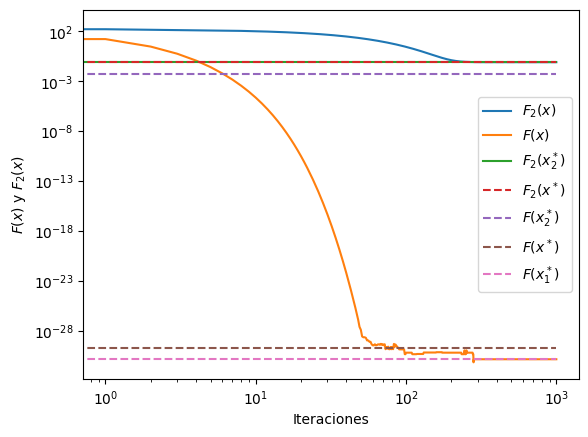
\includegraphics[width=0.8\textwidth]{f1 f2 iters.png}
    \caption{Evolución de la función de costo \(F(x)\) y \(F_2(x)\) en función de las iteraciones y resultados obtenidos  donde $x_1^*$ y $x_2^*$ son las respuestas obtenidas por el método de descenso por gradiente de la función $F(x)$ y $F_2(x)$ respectivamente despues de 1000 iteraciones y $x^*$ es la respuesta obtenida por SVD.}
    \label{fig:f1_f2}
\end{figure}

En la Figura \ref{fig:f2_delta} se muestra la evolución de la función de costo \(F_2(x)\) al variar el valor de \(\delta\) en el algoritmo de descenso por gradiente con regularización L2. Observamos que a medida que aumenta el valor de \(\delta\), la función de costo \(F_2(x)\) aumenta, lo que indica que la regularización L2 está penalizando más la norma de \(x\). Esto demuestra que el parámetro de regularización \(\delta\) controla la influencia de la regularización en la solución final. Cuanto mas se asemeje $\delta \approx 0, F_2(x) \approx F(x)$. En la Figura \ref{fig:f2_delta}, se elevaron al cuadrado la cantidad de iteraciones para mostrar la convergencia de los  distintos valores de $\delta$


\begin{figure}[H]
    \centering
    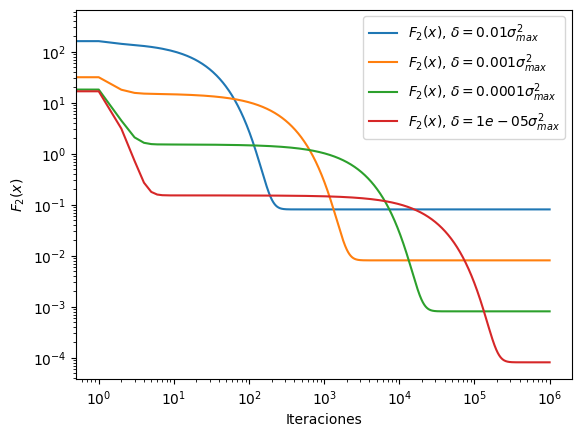
\includegraphics[width=0.8\textwidth]{vary delta f2.png}
    \caption{Evolución de la función de costo \(F_2(x)\) usando gradiente descendiente cambiando el valor de \(\delta\) con $1000^2$ iteraciones.}
    \label{fig:f2_delta}
\end{figure}

La figura \ref{fig:vectors} muestra la comparación de los vectores obtenidos por el método de descenso por gradiente y SVD. Observamos que los vectores obtenidos por el método de descenso por gradiente son similares a los obtenidos por SVD, lo que demuestra la efectividad del algoritmo en la resolución de sistemas lineales. Además, la regularización L2 mejora la precisión de la solución y evita el sobreajuste en sistemas mal condicionados.

\begin{figure}[H]
    \centering
    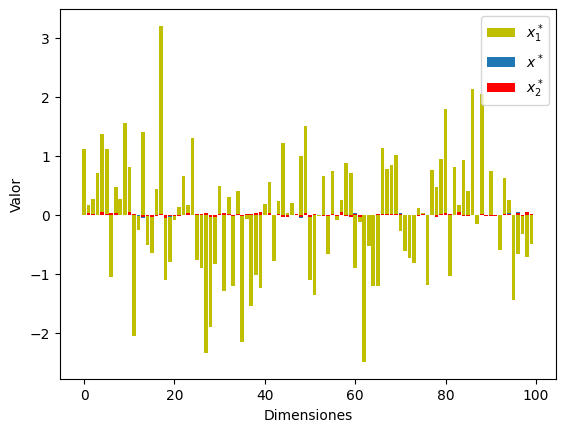
\includegraphics[width=0.8\textwidth]{vectors.png}
    \caption{Comparación de los vectores obtenidos por el método de descenso por gradiente y SVD.}
    \label{fig:vectors}
\end{figure}
En resumen, los resultados obtenidos demuestran que el algoritmo de descenso por gradiente es efectivo en la resolución de sistemas lineales y que la regularización L2 puede mejorar la convergencia y la precisión de la solución. Además, el parámetro de regularización \(\delta\) permite controlar la influencia de la regularización en la solución final. Estos resultados son consistentes con la teoría y demuestran la utilidad de estos métodos en la optimización de sistemas lineales.

\section{Conclusión}

\appendix




\printbibliography



\end{document}